\section{Exercise 6: Home Assistant}
The last exercise is about \textit{Home Assistant}. 
There are several tasks defined in the sheet about how to setup and use some features of \textit{Home Assistant}.

\subsection{Task 1: Setup}
As \textit{Home Assistant} recommends to use a Raspberry Pi to run the \textit{Home Assistant} server 
which is in my opinion more realistic than using a local virtual machine, i decided to use a Raspberry Pi 3B+ 
to run the \textit{Home Assistant} server. Image belows shows the \textit{Home Assistant} setup after the system was 
installed like described \href{https://www.home-assistant.io/installation/raspberrypi}{\textit{here}}.

\begin{figure}[H]
    \centering
    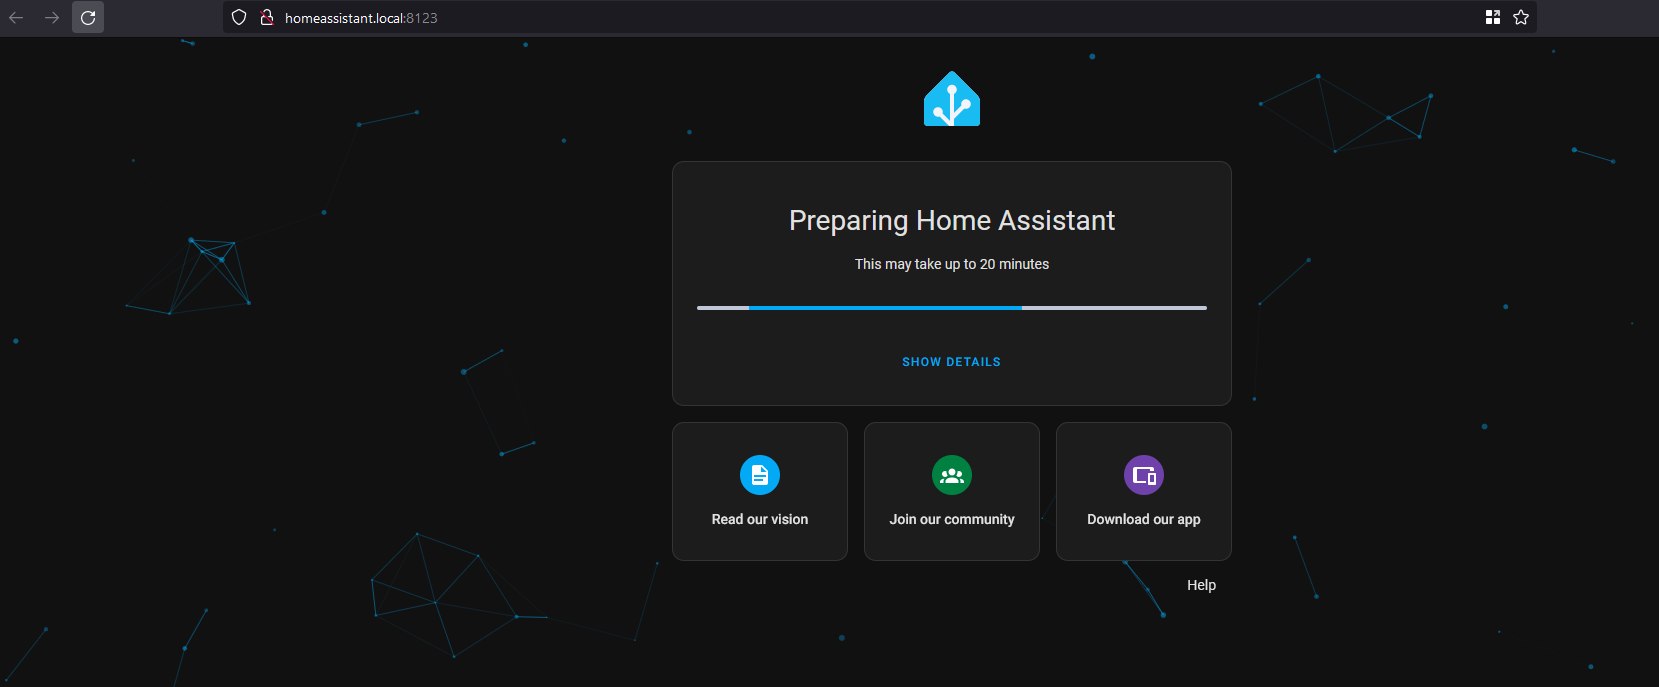
\includegraphics[width=1\textwidth]{exercise_home-assistant/setup.png}
    \caption{Home Assistant Setup}
    \label{fig:home_assistant_setup}
\end{figure}

After the setup was done the dashboard will be shown as seen in the image below.

\begin{figure}[H]
    \centering
    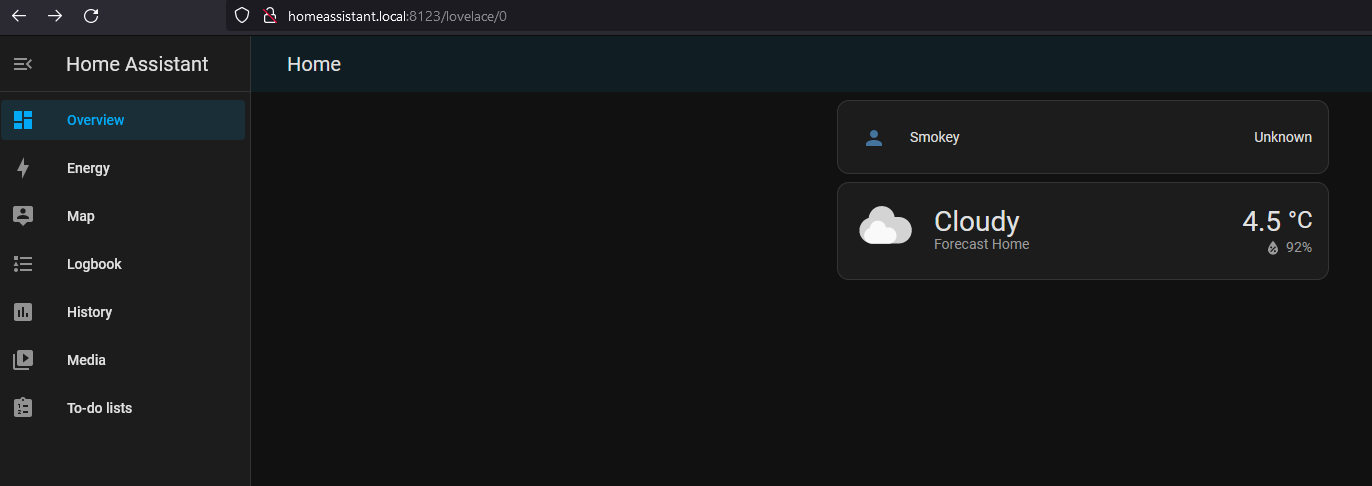
\includegraphics[width=1\textwidth]{exercise_home-assistant/dashboard_blank.png}
    \caption{Home Assistant Dashboard}
    \label{fig:home_assistant_dashboard}
\end{figure}

\subsection{Task 2: Add first service}
As first service it is required to add the \textit{AccuWeather} service to \textit{Home Assistant}.
This was mainly done like described in the tutorial \href{https://www.home-assistant.io/integrations/accuweather}{\textit{here}}.
Even if the default dashboard already contains a weather widget, i added this one to the dashboard as well.
Images below shows the successfully created \textit{AccuWeather Service} and the dashboard with the new widget.

\begin{figure}[H]
    \centering
    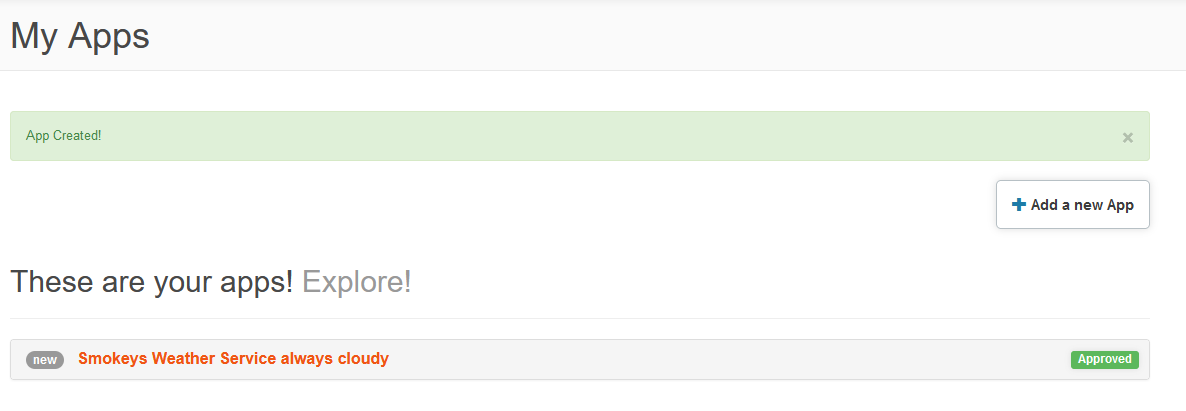
\includegraphics[width=1\textwidth]{exercise_home-assistant/accuweather.png}
    \caption{Home Assistant AccuWeather Service}
    \label{fig:home_assistant_accuweather_service}
\end{figure}

\begin{figure}[H]
    \centering
    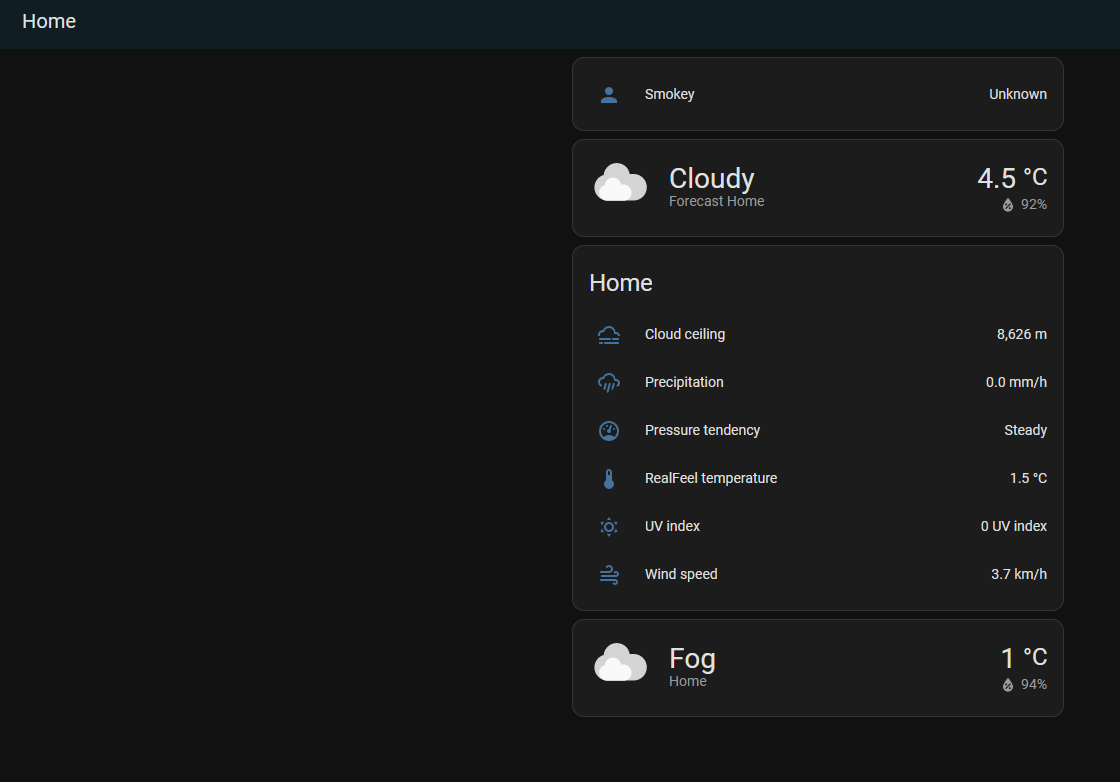
\includegraphics[width=1\textwidth]{exercise_home-assistant/dashboard_accuweather.png}
    \caption{Home Assistant Dashboard with AccuWeather Widget}
    \label{fig:home_assistant_dashboard_accuweather}
\end{figure}

\subsection{Task 3: Add first automation}
The third task is about adding the first automation to \textit{Home Assistant}.
Therefore it will be required to create a Telegram bot and add it to \textit{Home Assistant}. As i am not using 
Telegram i decided to use the \textit{Discord} bot instead. This was done like described in the tutorial 
\href{https://www.home-assistant.io/integrations/discord}{\textit{How to add discord bot}}.

After creating the new Discord application as described it will be shown in the Discord developer portal like 
shown in the image below.

\begin{figure}[H]
    \centering
    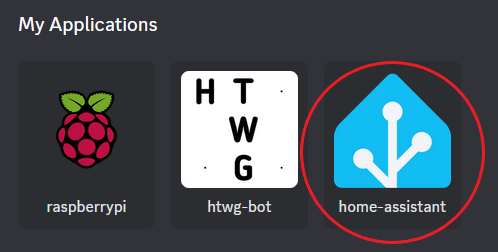
\includegraphics[width=1\textwidth]{exercise_home-assistant/discord_app.png}
    \caption{Discord Bot App View}
    \label{fig:discord_bot}
\end{figure}

After adding the Discord bot to \textit{Home Assistant} via the \textit{Devices & services Integration} and to a 
private Discord server i used other bots before i was able to create a first automation.
Therefore the \textit{Developer Tools} were used to change the \textit{notification} service like shown in the 
image below.

\begin{figure}[H]
    \centering
    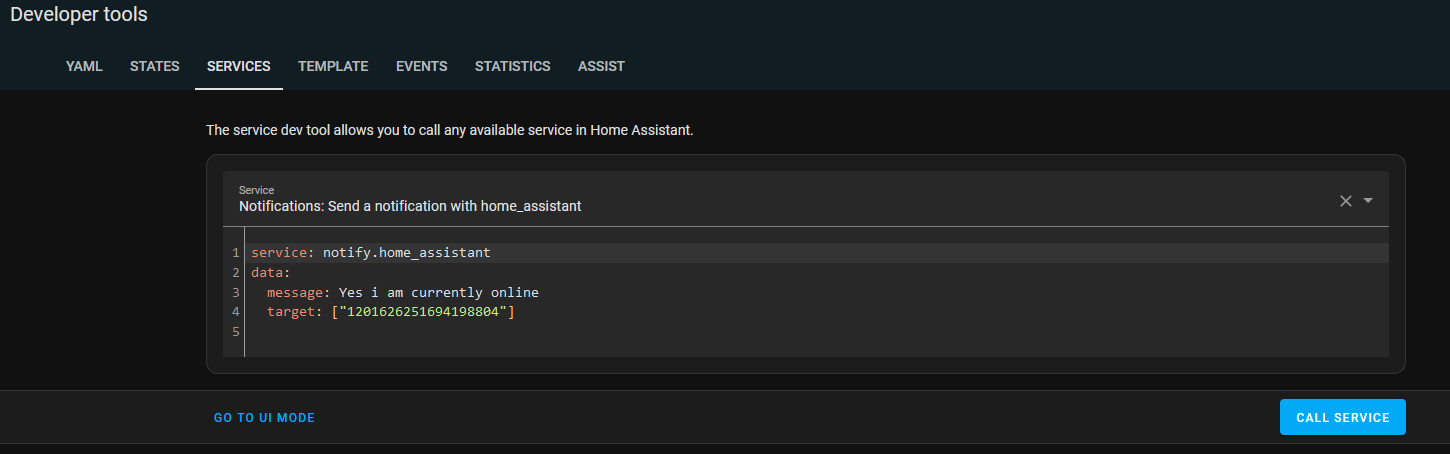
\includegraphics[width=1\textwidth]{exercise_home-assistant/service_yaml.png}
    \caption{Home Assistant Notification Service}
    \label{fig:home_assistant_notification_service}
\end{figure}

The target which is used in the \textit{target} field is the channel id of the channel where the Discord bot will 
send the messages to. Testing the service via the \textit{Call Service} button will send a message to the Discord 
channel like shown in the image below.

\begin{figure}[H]
    \centering
    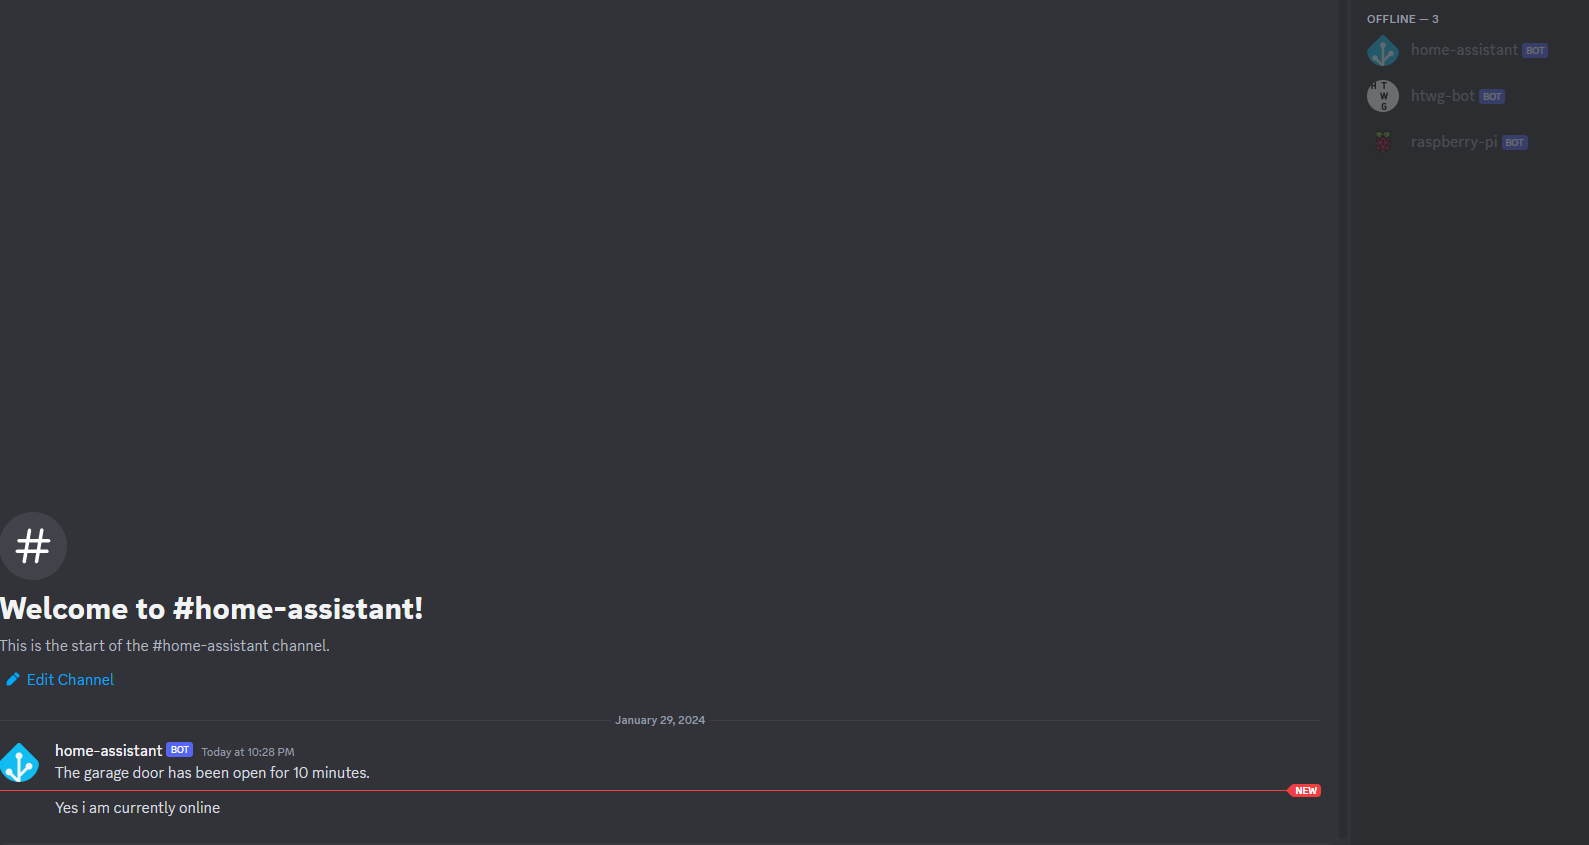
\includegraphics[width=1\textwidth]{exercise_home-assistant/bot_message.png}
    \caption{Discord Message from Home Assistant}
    \label{fig:discord_message}
\end{figure}


\subsection{Task 4: Add a periodical automation}
The fourth task is about adding a periodical automation to \textit{Home Assistant}.
Therefore the previous created notification service will be used to send a message to the Discord channel periodically.
Therefore I decided to use a message pattern like shown in the image bellow which will check the sun state and read the 
temperature data from the \textit{AccuWeather} service.
At the current version the notification will be send only once at minute 5 of every hour but can easily be extended to 
send the message every 5 minutes or every hour by adding more \textit{trigger} sections to the automation.

\begin{minted}
  [
    frame=lines,
    framesep=2mm,
    baselinestretch=1.2,
    linenos
  ]
  {C}

  trigger:
  - platform: time_pattern
    minutes: "5"
  - platform: time_pattern
    minutes: "10"
  ...
\end{minted}

The result of the automation can be seen in the image below as well as the discord notification which was send to the 
channel.

\begin{figure}[H]
    \centering
    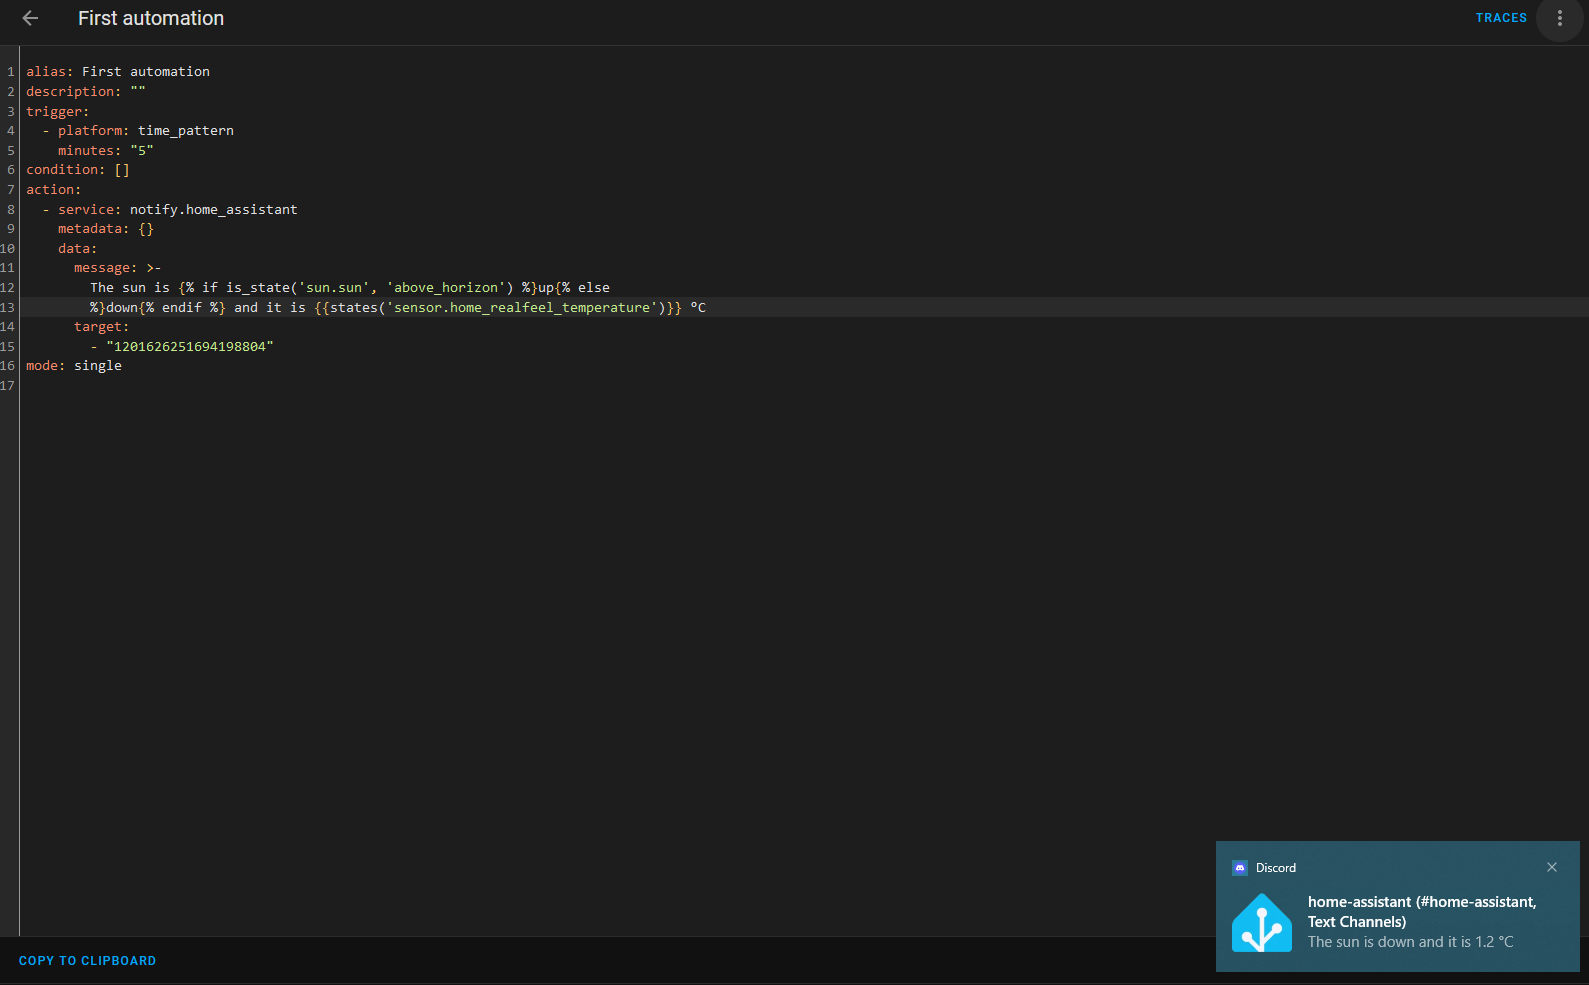
\includegraphics[width=1\textwidth]{exercise_home-assistant/automation.png}
    \caption{Discord Periodical Message from Home Assistant}
    \label{fig:discord_periodical_message}
\end{figure}

\subsection{Task 5: Smart Home Planning}
The last task is about planning a smart home system.
Therefore it was required to create floor plans for at least a basement floor as well as a ground floor and a first floor.
First i decided to create a floor plan using a online tool but most tools i found would need a little bit more time to 
get used to them. Therefore i decided to use the well known tool \textit{Paint} to create the floor plans.

\subsubsection{Import Floor Plan}
To use the floor plans in \textit{Home Assistant} it is required to import them as image files.
Therefore i created a new folder \textit{www} in the \textit{Home Assistant} configuration folder and copied the images 
into this folder. This was done using the \textit{Studio Code Server} extension which makes it possible to use the 
\textit{Visual Studio Code} editor in the browser and furthermore makes it easy to create and edit files in the 
\textit{Home Assistant} configuration folder.

After importing the images and restarting the \textit{Home Assistant} server the images can be used in the 
\textit{Home Assistant} dashboards. I would renewcommand to set the \textit{panel\_custom} configuration to 
\textit{true} to make it possible to use the images as background images for the dashboards (so they are not compressed).

\subsubsection{Device List}
To make a interactive floor plan using badges it would be required to add all devices to the \textit{Home Assistant} to 
control them. As i do not have any smart home devices i decided to just mark the devices in the floor plan like shown bellow.
As an example there is an badge added to the ground floor using the available sun sensor.

\begin{figure}[H]
    \centering
    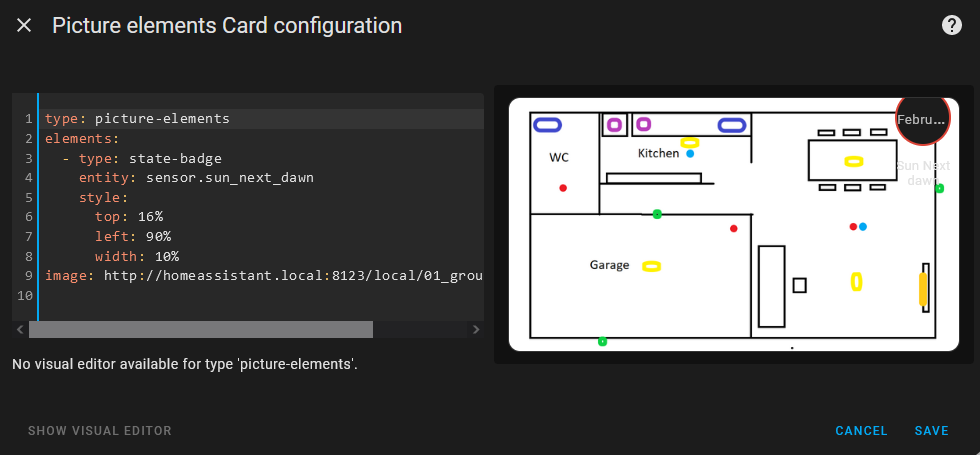
\includegraphics[width=1\textwidth]{exercise_home-assistant/example_badge.png}
    \caption{Ground Floor with Badges}
    \label{fig:ground_floor_badges}
\end{figure}

The following list shows the devices which are used in the floor plans.
As it is designed as that all devices are connected to the power grid (not using batterys),  all devices are connected via 
WiFi.

\begin{table}[!ht]
  \centering
  \begin{tabular}{|l|l|l|}
  \hline
      Color & Device & Connection \\ \hline
      Red & Smoke Detector & WiFi \\ \hline
      Green & Security Entry Devices & WiFi \\ \hline
      Blue & Smart Environment Controller & WiFi \\ \hline
      Light Blue & Smart Environment Sensor (Temperature, Humidity, CO2) & WiFi \\ \hline
      Yellow & Smart Lightning System & WiFi \\ \hline
      Orange & Smart Entertainment System & WiFi \\ \hline
      Purple & Smart Power Consumption System & WiFi \\ \hline
  \end{tabular}
\end{table}

Because of my good experience using \texit{MQTT} which was also used for my final project i would use \textit{MQTT} to 
connect all devices to the \textit{Home Assistant} server. This would make it possible to use the \textit{MQTT} broker 
to connect all devices to the \textit{Home Assistant} server and furthermore make it possible to use the \textit{MQTT} 
broker to connect the \textit{Home Assistant} server to other services like \textit{Node-RED}.

\subsubsection{Ground Floor}
The ground floor is designed as the main living area at will be the first page of the dashboard.

\begin{figure}[H]
    \centering
    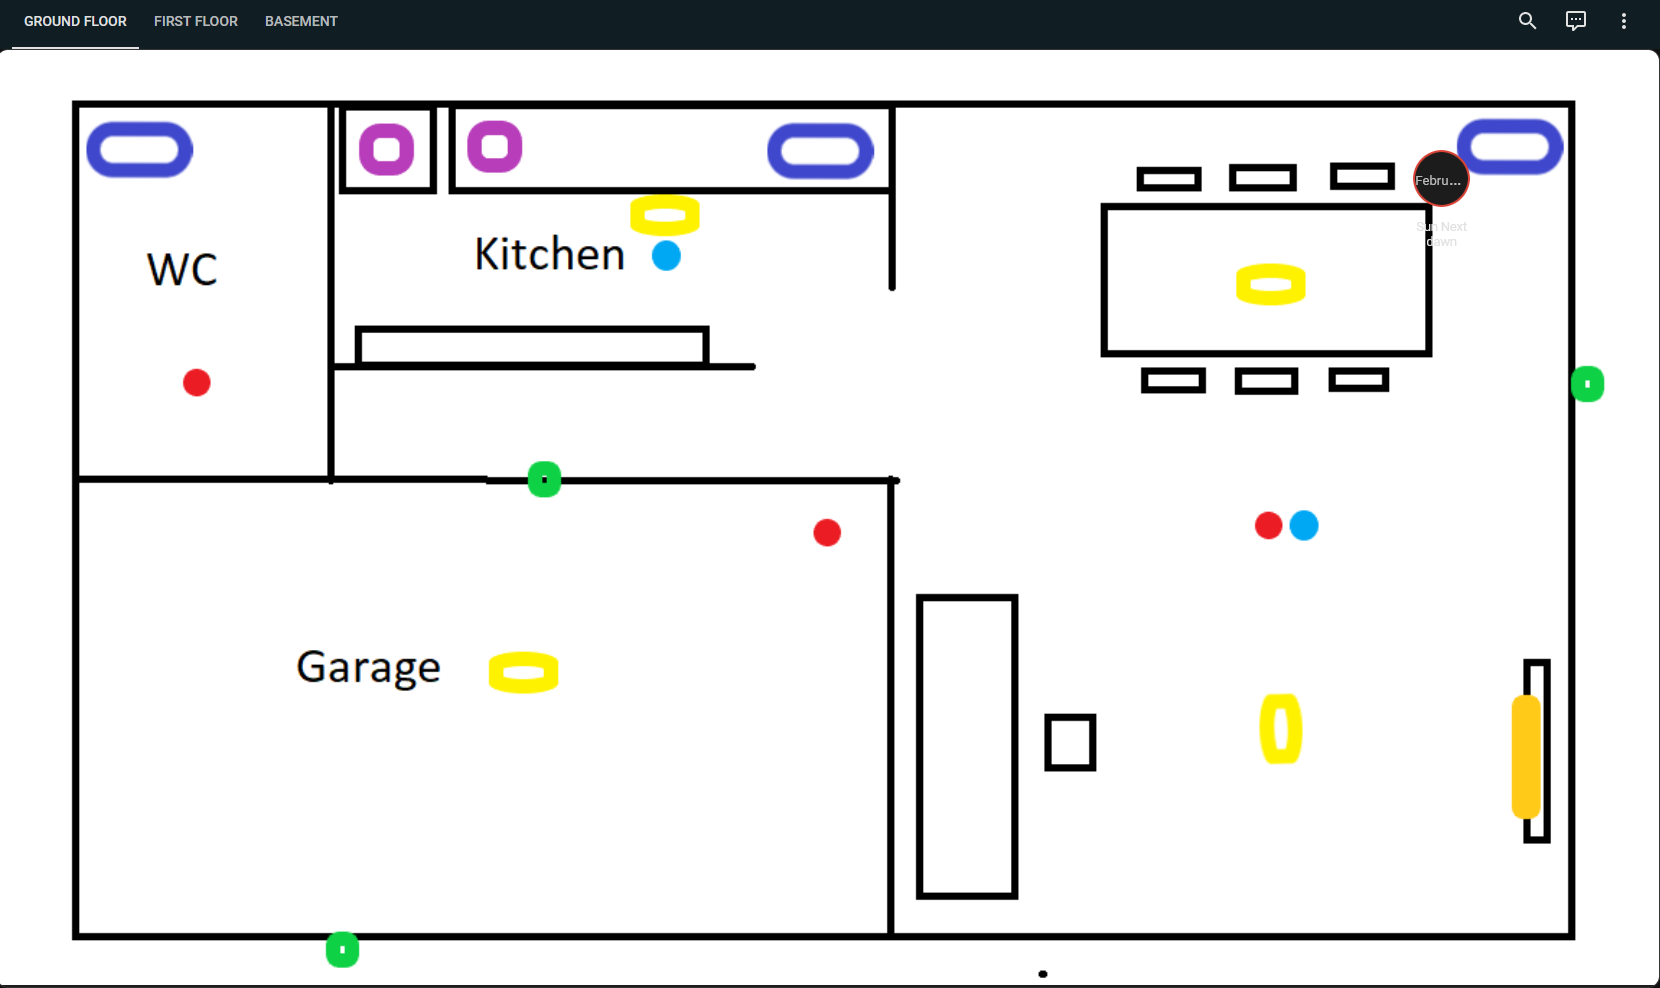
\includegraphics[width=1\textwidth]{exercise_home-assistant/plan_ground_floor.png}
    \caption{Ground Floor}
    \label{fig:ground_floor}
\end{figure}

\subsubsection{First Floor}
The first floor is designed as the sleeping area and will be the second page of the dashboard.

\begin{figure}[H]
    \centering
    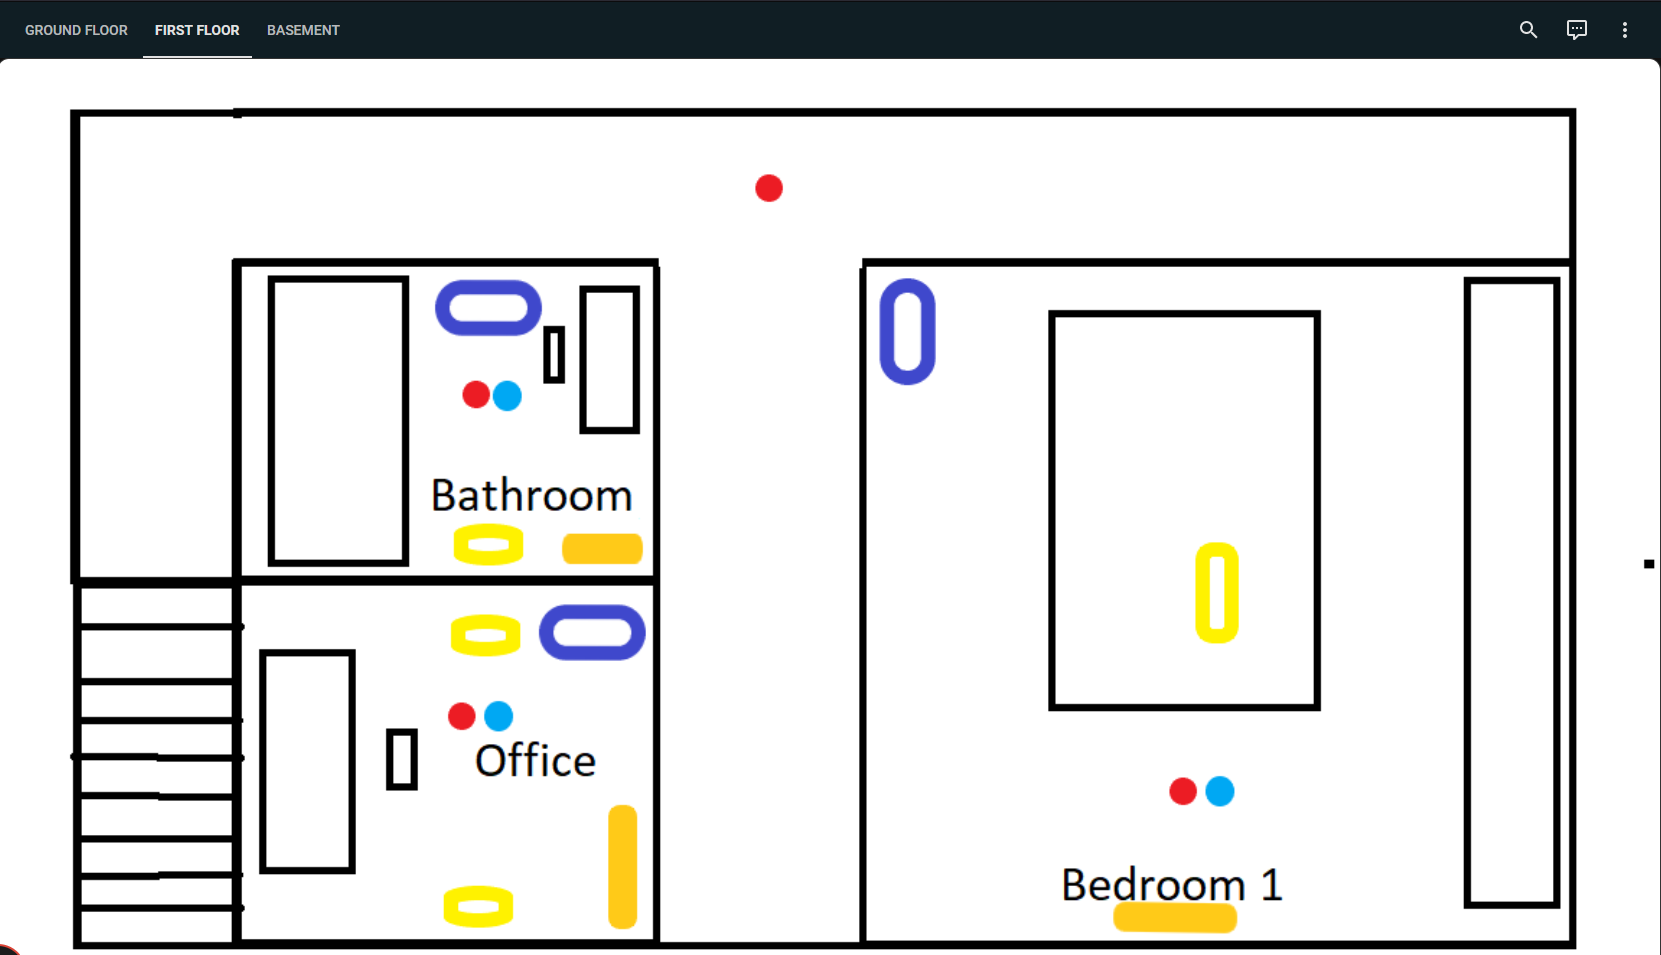
\includegraphics[width=1\textwidth]{exercise_home-assistant/plan_first_floor.png}
    \caption{First Floor}
    \label{fig:first_floor}
\end{figure}

\subsubsection{Basement Floor}
The basement floor is designed as the cleaning and workbench area and will be the third page of the dashboard.

\begin{figure}[H]
    \centering
    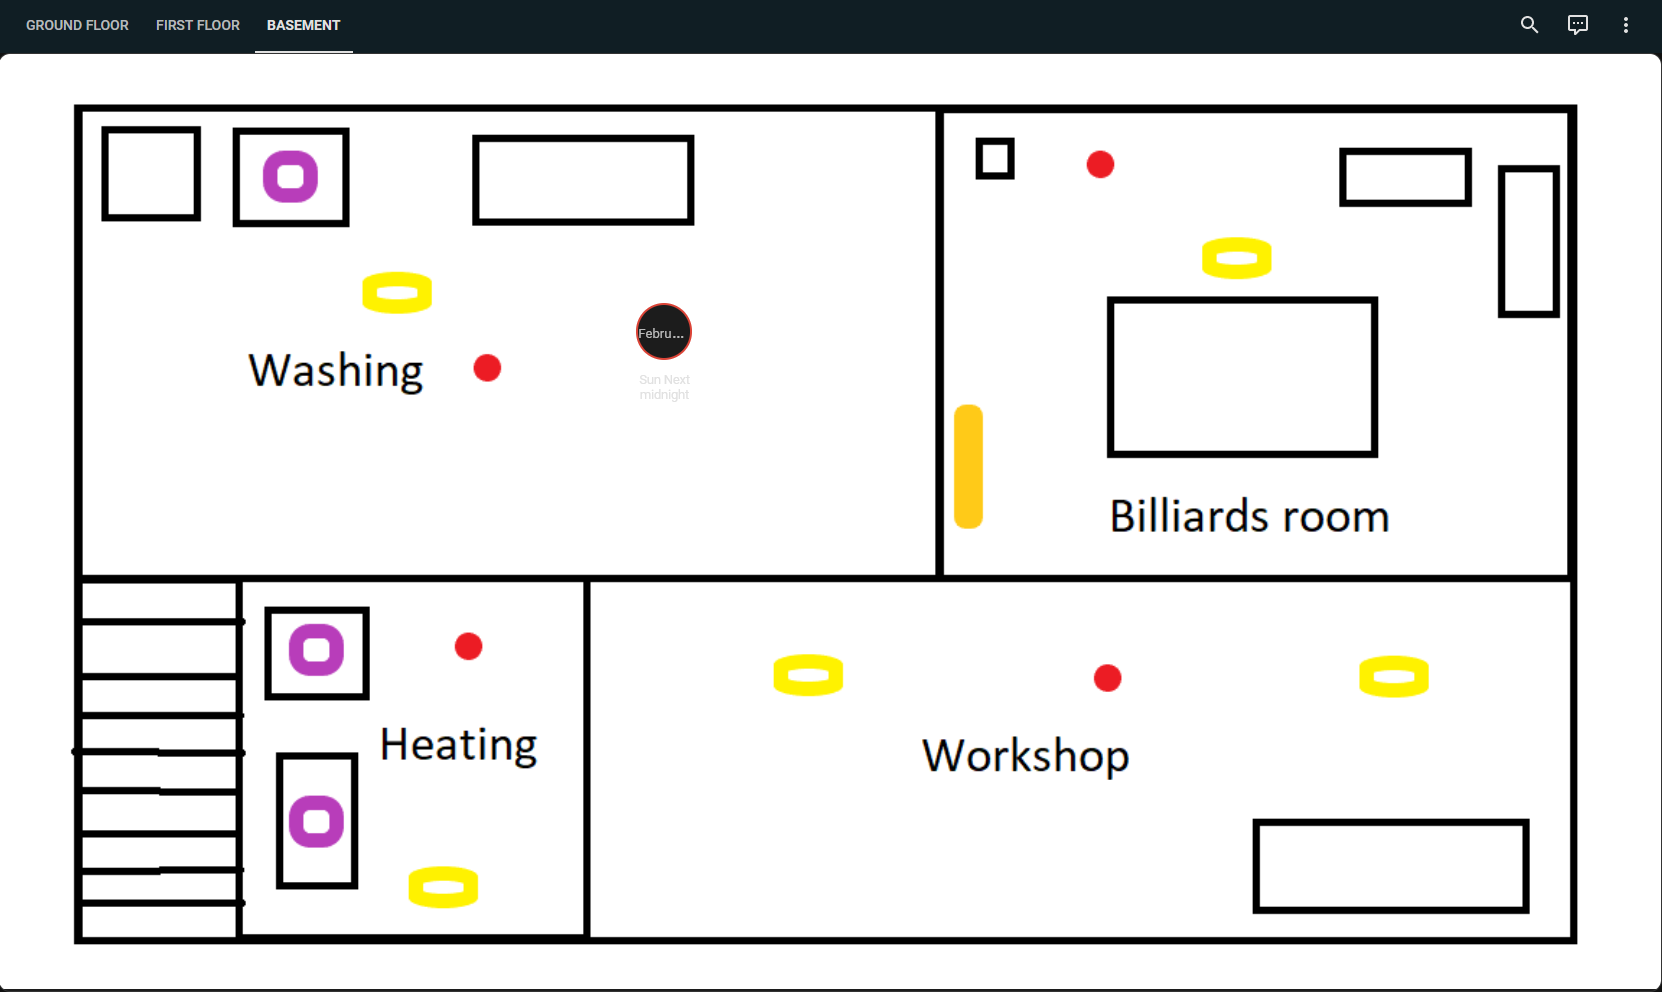
\includegraphics[width=1\textwidth]{exercise_home-assistant/plan_basement_floor.png}
    \caption{Basement Floor}
    \label{fig:basement_floor}
\end{figure}

\subsubsection{Sensors}

\subsubsubsection{Smoke Detector}
The smoke detector is designed to detect smoke and fire and will be connected to the \textit{Home Assistant} server 
using \textit{MQTT}. It should be possible to check the status of the smoke detector using the dashboard as well as 
turning them on and off. Furthermore it should be possible to get a notification if the smoke detector detects smoke or 
fire. On one side they should notice via alarm sound as well as via notification on the dashboard and via notification 
on the previously created Discord bot.

\subsubsubsection{Security Entry Devices}
The security entry devices are designed to detect if a door or window is opened or closed and will be connected to the 
\textit{Home Assistant} server using \textit{MQTT}. It should be possible to check the status of the security entry 
devices using the dashboard. Like already realized in the final project finger print sensors should be used to 
authenticate the user. Turn the system on and off should be possible using the dashboard as well as using a 
command send to the Discord bot.

\subsubsubsection{Smart Environment Sense}
The smart environment sense is designed to measure the temperature, humidity and CO2 level in the room and will be 
connected to the \textit{Home Assistant} server using \textit{MQTT}. It should be possible to check the status of the 
smart environment sense using the dashboard. Furthermore it should be possible to get a notification if the CO2 level 
is to high.

\subsubsubsection{Smart Environment Controller}
The smart environment controller is designed to control the heating, cooling and ventilation system and will be 
connected to the \textit{Home Assistant} server using \textit{MQTT} as well.
It should be possible to control the heating, cooling and ventilation system using the dashboard for 
example to set the temperature or turn the system on and off.

\subsubsubsection{Smart Lightning System}
The smart lightning system is designed to control the lights in the rooms.
It should be possible to control the lights using the dashboard for example to turn the lights on and off or to change 
the brightness of the lights. As already mentioned in the final project presentation this should only be "IoT as a 
feature" meaning that it should be possible to control the lights using the dashboard but it should also be possible to 
control the lights using physical switches.

\subsubsubsection{Smart Entertainment System}
The smart entertainment system is designed to control the entertainment system in the rooms like the TV or the HiFi.
It should be possible to control the entertainment system using the dashboard for example to play music or to turn the 
TV on and off.

\subsubsubsection{Smart Power Consumption System}
The smart power consumption system is designed to measure the power consumption of some devices like the Heating, 
Cooling or Kitchen devices. It should be possible to check the power consumption of the devices using the dashboard 
but also to export the data to a file to analyze the data like done in exercise 4.